% I've put this section first so the later chapters can already rely on the reader knowing what the scenario is about. Furthermore, we can then directly rule out concepts which we are presenting by applying them theoretically onto the scenario/our needs.
This section and its subsections introduce the Multi-Agent Programming Contest (short: \emph{MAPC}).
It is an international online competition which started in 2005 and took place every year since then.
This tournament is held as an online event in the sense that all participants run their systems locally and communicate with the contest server via Internet.
The winning team is determined by each team playing against all other teams three times.
All participants are free to choose which technologies and implementations they want to use for building their multi-agent system upon.
The scenario of the MAPC has changed several times over the years:
\begin{itemize}
	\item 2005: Food Gatherers
	\item 2006-07: Gold miners
	\item 2008-10: Cows and Cowboys
  \item Since 2011: Agents on Mars
\end{itemize}
The scenarios became more and more complex as the agents' features were extended and heterogeneous agent roles were added~\cite{behrens_multi-agent_2012}. % 113

\autoref{fun:mapc_general} describes 2014's \mars{} briefly.
It covers the story motivating the scenario, the goals of the scenario and the representation of the environment.
Furthermore, it presents how team scores are calculated in the competition.
\autoref{fun:mapc_roles} addresses the agents and the actions which they may execute.
The focus of the section is to explain all executable actions and their effects.
Thereby, the agent-specific roles of the \mars{} and their differences are covered.

\subsubsection[The \mars{}]{The \mars{}$^{\odot,\circ}$}\label{fun:mapc_general}
This section presents the \mars{}.
A detailed description of it can be found in Ahlbrecht et~al.~\cite{ahlbrecht_mapc_2014}.
Briefly, mankind finally populated Mars and water wells have been found.
One sub-goal is to occupy the most valuable water wells, and defend them against the competing team.
The environment is represented as a weighted graph.
Each vertex has a unique identifier and a positive number indicating the value of the well.
Edges have a weight each which represent the costs of traversing this edge.
The environment is unknown in the beginning and thus agents have to explore it.

\emph{Zones} are regions over one or multiple vertices which express the successful occupation of water wells by a team.
They are determined by using a graph colouring algorithm on the server side which is presented in more detail in Ahlbrecht et~al.~\cite{ahlbrecht_mapc_2014}.
Essentially, a zone is identified as follows:
\begin{enumerate}
	\item A vertex belongs to the team which holds the majority of agents standing on that vertex.
	\item Vertices directly connected to at least two neighbours dominated by the same team also belong to that team.
	\item All vertices that are not reachable by other teams without crossing the already coloured vertices also belong to that team.
    One can see it as a border that	is separating parts of the graph.
\end{enumerate}

The overall goal is to maximise the team's score.
This score is calculated by adding the zones' values and the money for each simulation step as shown in \autoref{eq_score}.
\begin{equation}\label{eq_score}
  \sum_{k=1}^\textit{steps}\left(\textit{zones}_k + \textit{money}_k\right)
\end{equation}
Money is rewarded for achievements like successfully performing an action a certain number of times.
A team has two options for using its money.
It can either be spent to buy upgrades for an agent's attributes or it can be saved in order to increase the score per step.
In the subsequent section, the agents and their attributes are presented in more detail.


This section presents the basic behaviour of our agents given the actions that all agents share.
Every agent team in the MAPC Scenario consists of 28 agents.
These agents are divided into five roles: the Explorer agent, the Repairer agent, the Saboteur agent, the Sentinel Agent and the Inspector agent.
\begin{figure}[ht]
  \centering
  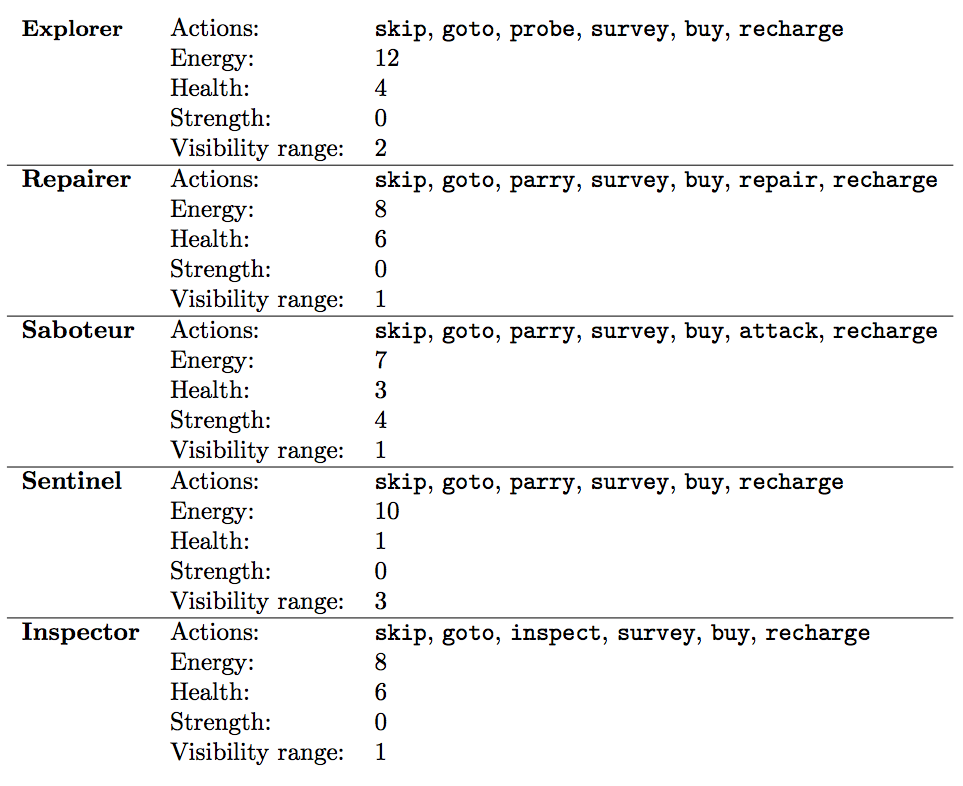
\includegraphics[width=0.9\linewidth]{images/roles.png}
  \caption{The different agent roles in the MAPC scenario \cite{ahlbrecht_mapc_2014}.}
  \label{fig:fun:roles}
\end{figure}
As shown in \autoref{fig:fun:roles}, each role is given different values in their attributes of maximum energy, health or visibility range.
Moreover, the saboteur agent has a strength value, because it is the only agent which can attack enemy agents.
There are six agents of each role except the Explorer agent role of which there are four agents.
Except for the Sentinel role, all other roles allow their corresponding agents to execute some actions exclusive to this role. 
Every action has a minimal chance to fail, regardless of being an exclusive action or an special action which is only available to the specific agent. 
Some actions can be executed on distant agents. They are called ranged actions. 
The drawback of ranged actions is that they have a much higher failing chance if the target of the action is further afar.
First, the actions all agents are able to execute will be presented. After that the exclusive actions of the agents will be described.
Those actions are \texttt{skip}, \texttt{goto}, \texttt{survey}, \texttt{buy} and \texttt{recharge}.
\begin{description}
   \item[skip] The \texttt{skip} action should be used as a last resort if there is nothing else for an agent left to do.
    This action's only purpose is to tell the server that an agent did not time out but was not interested in executing a different action.
    If the \texttt{skip} action is executed when an agent could have e.g. recharged instead, it can be seen as a wasted step for this particular agent.
   \item[goto] The \texttt{goto} action is used to traverse over edges from one vertex to another adjacent vertex.
    Said traversing is only possible when the costs of the edge to traverse are lower than or equal to the energy the agent currently has.
    Else, the execution of the method will fail.
    By successfully executing the \texttt{goto} action, the current energy of the agent is reduced by the traversing costs of the edge.
   \item[survey] When the ability \texttt{survey} is executed, weights of edges in the visibility range of the agent are retrieved.
    The count of edge weights an agent gets as percept is determined randomly based on the visibility range of the agent.
   \item[buy] With the action \texttt{buy} an agent is able to upgrade its values like maximum health and visibility range.
    Saboteur agents can furthermore increase their strength through this action.
   \item[recharge] If an agent has a low energy level the ability \texttt{recharge} fills up the energy of the agent.
    By each \texttt{recharge} action the current energy is recharged by half of the maximum energy.
\end{description}

The role specific actions are explained in the following. 
\begin{description}
   \item[parry] The \texttt{parry} action can be used by repairer agents, sentinel agents and saboteur agents. 
    By using the action an incoming attack can be fully neglected  and the health of the agent is preserved.
   \item[inspect] Only inspector agents can use the \texttt{inspect} action. Inspecting is a ranged action. 
    The action reveals the inner stats and details of the targeted agent. 
    By inspecting it is possible to find out which role an enemy agent has. 
    Inspecting is not needed to be able to tell if an agent is disabled as one could assume from the action's name. 
    This is because the \texttt{visibleEntity} percept includes the agent's current state.
   \item[repair] Repairing is an ranged action which is unique to repairer agents. The \texttt{repair} action repairs an agent of the same team. 
    Repairing can not be executed on the agent itself.
   \item[probe] Explorer agents are the only agents which can reveal the value of vertices with its \texttt{probe} action.
    As long as a vertex is not probed the vertex value is calculated as 1. Probing is an ranged action and thus can be executed on distant vertices.
   \item[attack] The \texttt{attack} action can only be executed by saboteur agents. It is used to attack an enemy agents and reduce its health by a specific amount until it gets disabled. Attacking is a ranged action.   
\end{description}

The use and embodiment of these unique abilities into the agent role specific behaviour is explained in \autoref{alg:agentstrategies}.

